\begin{frame}[label={lastslide}]{Conclusion and Perspectives}
	\begin{itemize}
		\item PINNs are good candidates for the enriched approach. \refappendix{frame:datavspinns}
		\item Numerical validation of the theoretical results.
		\item The enriched approach provides the same results as the standard FEM method, but with coarser meshes.
		$\Rightarrow$ Reduction of the computational cost.
	\end{itemize}

	\textbf{Perspectives :}

	\begin{itemize}
		\item Consider non-linear problems. %\refappendix{frame:nonlinear}
		\item Use PINN prediction to build an optimal mesh, via a posteriori error estimates.
		\item Validate the additive approach on more complex geometry.
		
		\centering
		\vspace{7pt}
		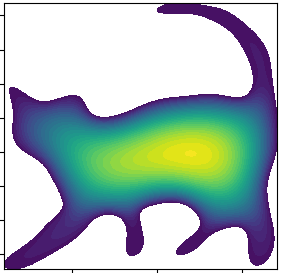
\includegraphics[width=0.3\linewidth]{images/conclu_cat.png}
	\end{itemize}
\end{frame}

